\documentclass[table]{beamer}
\usetheme{gpmeet}
\setbeamertemplate{caption}{\raggedright\insertcaption\par}
\graphicspath{{../../figures/}}

\newcommand{\leftRect}[2]{\node[draw=text,very thick,rounded corners, text width=0.46\textwidth,minimum height=6cm] at (0,0) {\centering\textbf{#1}\\ \raggedright \color{text}#2};}
\newcommand{\rightRect}[2]{\node[draw=text,very thick,rounded corners, text width=0.46\textwidth,minimum height=6cm] at (0.54\textwidth,0) {\centering\textbf{#1}\\ \raggedright \color{text}#2};}

\usepackage{tikz}

\title{Group meetings}

\subtitle{Memristors-based recurent modules for neural computing}

\author[V. BARBAZA]{Valentin BARBAZA}

\date{26/06/2023}

\logo{
  \begin{tikzpicture}[overlay,remember picture]
    \node[below=1pt] at (current page.55){
      
\includegraphics[height=1cm]{logos/ist}
      \hspace{1pt}
      
\includegraphics[height=1cm]{logos/inesc-mn.png}
      
\includegraphics[height=1cm]{logos/inesc-id.eps}
    };
  \end{tikzpicture}
  }

  \begin{document}

  \frame{\titlepage}


  \begin{frame}
    \frametitle{Introduction}

    \begin{itemize}
        \color{text}
      \item I am working on an analog implementation of a LSTM Neural Networks.
      \item The final objective of my thesis is to have a successful simulation of such a circuit.
    \end{itemize}

  \end{frame}


  \begin{frame}
    \frametitle{Introduction}
    \centering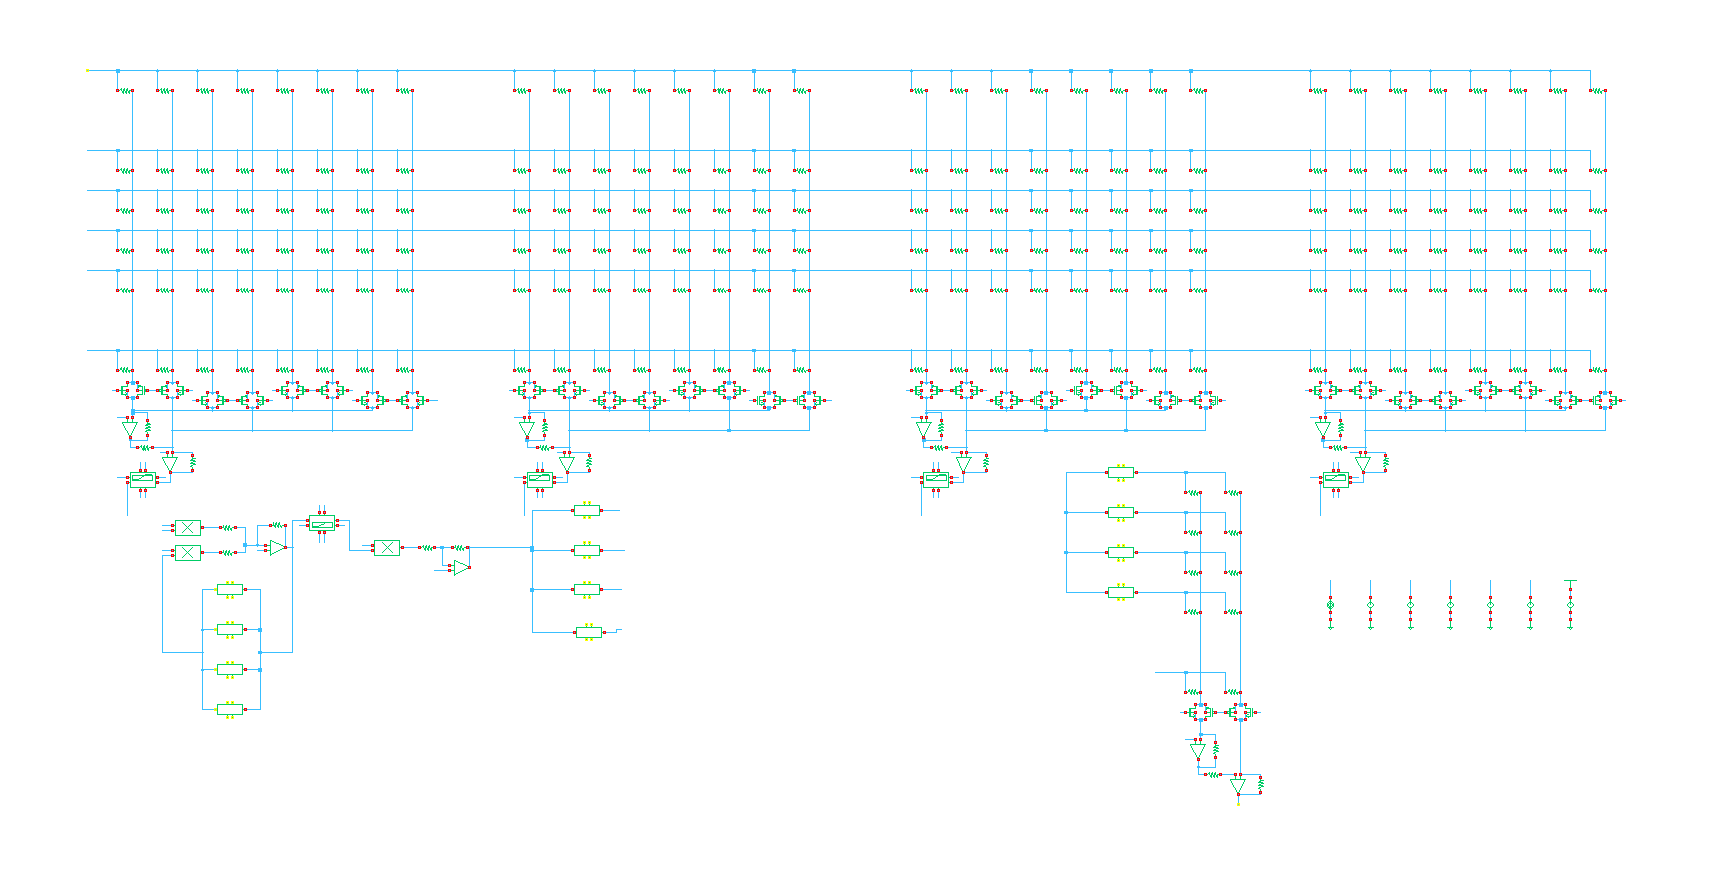
\includegraphics[width=\textwidth]{lstm/lstm-np}
  \end{frame}

  \begin{frame}
    \frametitle{Last weeks...}

    Last meeting, I promised to do :

    \centering
    \rowcolors{2}{evenRow}{oddRow}
    \begin{tabular}{c p{0.3\textwidth} c p{0.3\textwidth} c}
      \rowcolor{firstRow}
      \color{white}\textbf{\#} & \centering\color{white}Task & \color{white}Done? & \color{white}Why not? & \color{white}Help? \\
      1 & Find another LSTM problem & On going & Didn't find & Yes\\
      2 & Find out what is causing the issue & Partly & I had a scale of 10000 and reduced it to 1.5 & No\\
      3 & Find formula for approximate onChip area & No & Can be done later & No\\
      4 & Work on thesis & On going & & No\\
    \end{tabular}

  \end{frame}

  \begin{frame}{What's new}
    \begin{itemize}
      \item Results obtianed :
        \begin{itemize}
            \color{text}
          \item I reduced the factor of the results
          \item The factor is now tolerable, will have to see how it behaves with other problems
        \end{itemize}
      \item Improvements :
        \begin{itemize}
            \color{text}
          \item Reduce the still existing factor
        \end{itemize}
      \item Relevant information :
        \begin{itemize}
            \color{text}
          \item I reduced the factor to 16 first, and then to 1.5.
        \end{itemize}
    \end{itemize}
  \end{frame}

  \begin{frame}{What's new}
    Here the scale factor is almost the same with the serialized and parallel version (1.50 vs 1.58).
    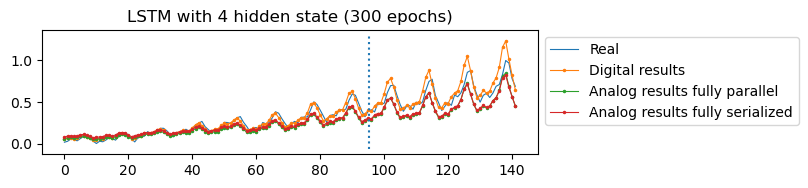
\includegraphics[width=\textwidth]{output/factor1.5.png}
  \end{frame}

  \begin{frame}{What's new}
    Today, I managed to reduce the scale factor even more. (1.21)
    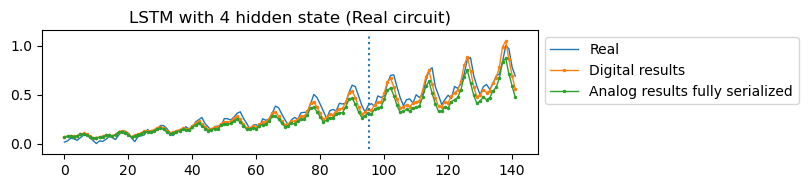
\includegraphics[width=\textwidth]{output/factor1.2.png}
  \end{frame}

  \begin{frame}
    \frametitle{Problems/doubts}
    \begin{itemize}
      \item The results are still not quite right.
      \item I am wondering whether it is still due to the activation function circuit.
    \end{itemize}
  \end{frame}

  \begin{frame}{Problems/doubts}
    I had to train using custom activation function but still not perfect.
    \begin{figure}[!tbp]
      \centering
      \begin{minipage}[b]{0.4\textwidth}
        \centering
        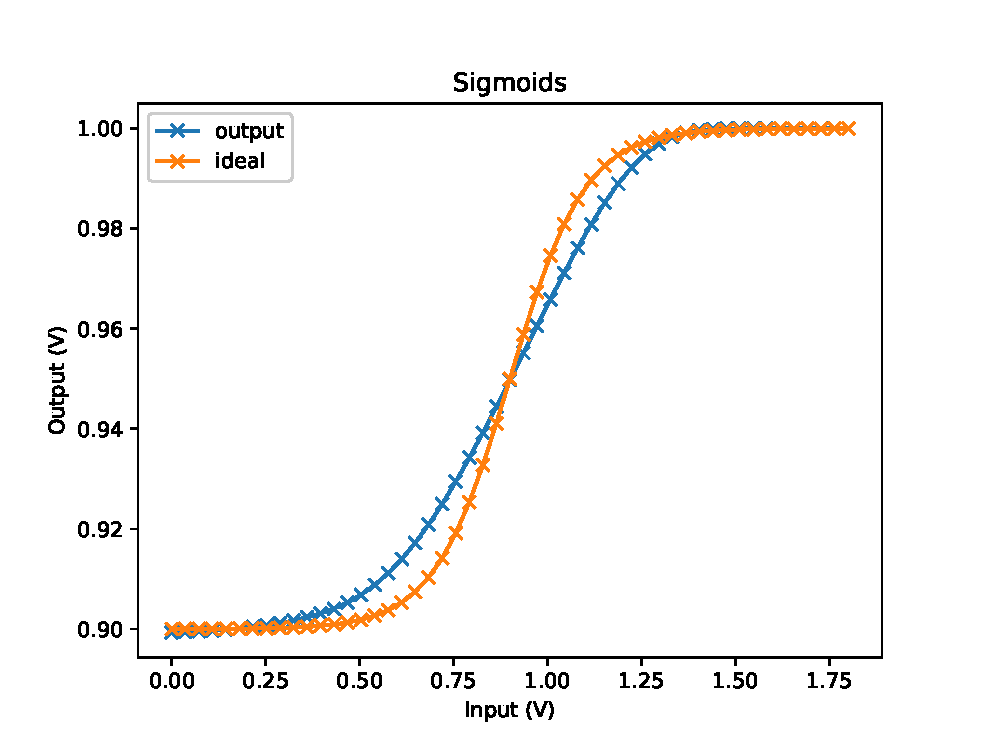
\includegraphics[width=\textwidth]{activation/sigmoid}
        \caption{ $Sigmoid(x)$ - RSME : 0.0051}
      \end{minipage}
      \hspace{20pt}
      \begin{minipage}[b]{0.4\textwidth}
        \centering
        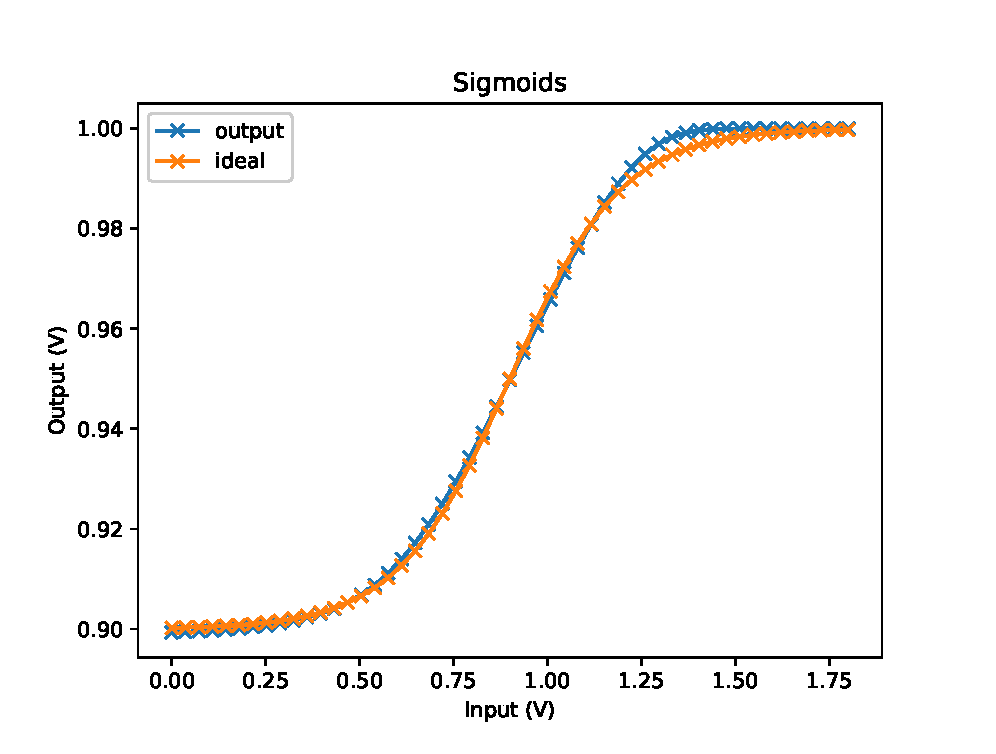
\includegraphics[width=\textwidth]{activation/cSigmoid}
        \caption{ $ Sigmoid(0.67\cdot x) $ - RSME : 0.0014}
      \end{minipage}
      \caption{Sigmoid}
    \end{figure}
  \end{frame}

  \begin{frame}{Problems/doubts}
    I had to train using custom activation function but still not perfect.
    \begin{figure}[!tbp]
      \centering
      \begin{minipage}[b]{0.4\textwidth}
        \centering
        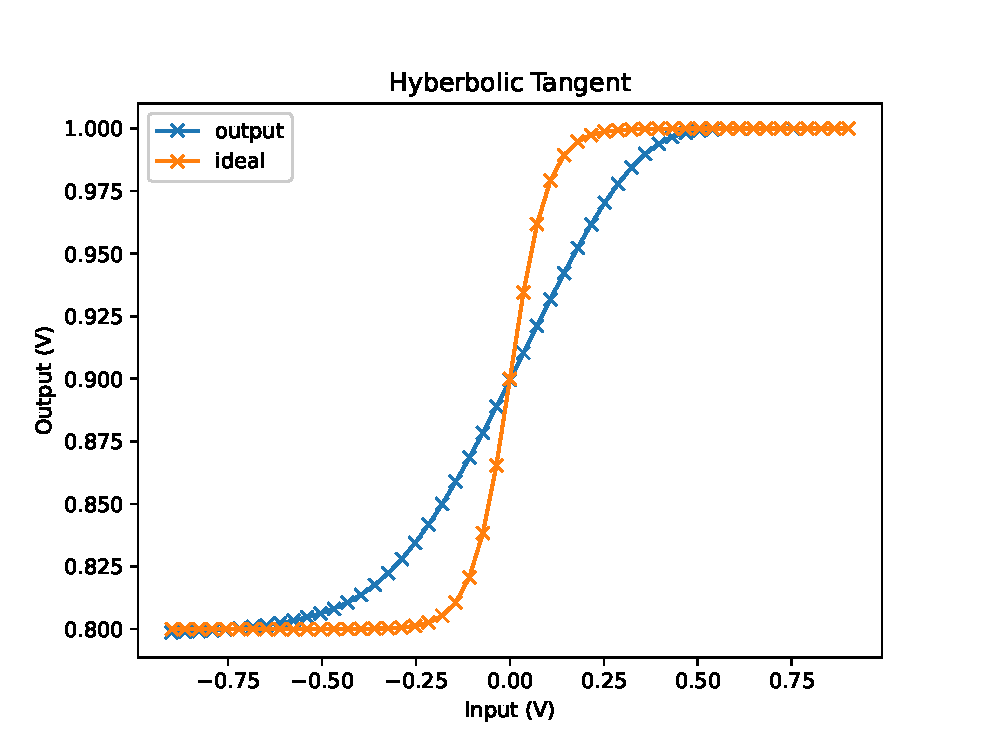
\includegraphics[width=\textwidth]{activation/tanh}
        \caption{ $ Tanh(x) $ - RSME : 0.022}
      \end{minipage}
      % \rightarrow
      \hspace{20pt}
      \begin{minipage}[b]{0.4\textwidth}
        \centering
        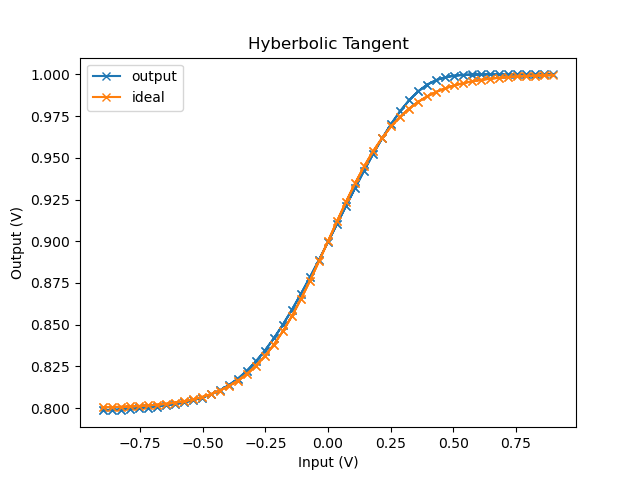
\includegraphics[width=\textwidth]{activation/cTanh}
        \caption{ $2\cdot Sigmoid(0.67\cdot x)-1$ - RSME : 0.0029}
      \end{minipage}
      \caption{Tanh}
    \end{figure}
  \end{frame}

  \begin{frame}{Next weeks}

    List of what I plan to do in the next weeks :

    \centering
    \rowcolors{2}{evenRow}{oddRow}
    \begin{tabular}{ c m{6cm} }
      \rowcolor{firstRow}
      \color{white}\textbf{\#} & \centering\color{white}Task \cr
      0 & Work on thesis \\
      0.1 & Formula onChip Area \\
      1 & Find another LSTM problem \\
      2 & Try to reduce the scale factor again \\
      2.1 & Tensorflow custom function \\
    \end{tabular}
  \end{frame}

  \begin{frame}{Networking and sharing}
    \begin{tikzpicture}
      \leftRect{Help/Collaboration :}{- If anybody has any idea of an interesting LSTM/NN problem to work on.}

      \rightRect{Recommendations :}{None}
    \end{tikzpicture}
  \end{frame}

\end{document}
